\chapter{Superpixel Segmentation}
\label{chapter:superpixel-segmentation}

We devote this chapter to reviewing two state-of-the-art algorithms to generate superpixel segmentations from color images: \textbf{SEEDS} \cite{VanDenBerghBoixRoigCapitaniVanGool:2012} and \textbf{SLIC} \cite{AchantaShajiSmithLucchiFuaSuesstrunk:2010}. While \textbf{SEEDS} represents the main focus of this thesis, \textbf{SLIC} is introduced for two reasons. Firstly, it offers a natural extension to depth and secondly, it is commonly used as baseline and especially popular because of its simplicity. In addition, other approaches like \textbf{DASP} \cite{WeikersdorferGossowBeetz:2012} and \textbf{VCCS} \cite{PaponAbramovSchoelerWoergoetter:2013}, discussed in chapter \ref{chapter:superpixel-segmentation-depth}, have strong similarities to \textbf{SLIC}.

\section{SEEDS}
\label{section:superpixel-segmentation-seeds}

\textbf{SEEDS} is a gradient ascent method which, in contrast to other methods as \textbf{SLIC} or \textbf{TP} \cite{LevinshteinStereKutulakosFleetDickinsonSiddiqi:2009}, starts with an initial superpixel segmentation and iteratively refines it to maximize an energy \cite{VanDenBerghBoixRoigCapitaniVanGool:2012}. As the actual implementation differs from the algorithm proposed by Van den Bergh \etal, we first discuss the algorithm in detail before introducing the theoretical background.

\subsection{Algorithm}
\label{subsection:superpixel-segmentation-seeds-algorithm}

The algorithm begins with grouping pixels into blocks of size $w^{(1)} \times h^{(1)}$ (\eg $2 \times 2$, $2 \times 3$, $3 \times 2$, \dots). These blocks are then further arranged in groups of $2 \times 2$. This can be applied recursively to form a hierarchy of blocks such that blocks at level $l$ have size $w^{(l)} \times h^{(l)}$ with
\begin{align}
	w^{(l)} = w^{(1)}\cdot 2^{l-1}\quad\text{ and }\quad h^{(l)} = h^{(1)}\cdot 2^{l-1}.
\end{align}
For a total of $L$ levels, the blocks at level $L$ represent the initial superpixels. Therefore, the number of superpixels is calculated as
\begin{align}
	K = \floor*{\frac{W}{w^{(L)}}} \cdot \floor*{\frac{H}{h^{(L)}}}.
\end{align}
This means that the minimum block size $w^{(1)} \times h^{(1)}$ and the number of levels $L$ need to be derived from the desired number of superpixels $K$ and the image size $W \times H$.

The initial superpixel segmentation is refined by exchanging blocks or pixels between neighboring superpixels. Blocks are exchanged based on their similarity to the respective superpixel expressed as histogram intersection. Therefore, let $B_i^{(l)} \subseteq \ubar{W} \times \ubar{H}$ be a block of pixels at level $1 \leq l < L$ and $S_j$ be a superpixel. Further, let $h_{B_i^{(l)}}$ denote the color histogram of block $B_i^{(l)}$ such that $h_{B_i^{(l)}}(q)$, $1 \leq q \leq Q$, is the fraction of pixels within $B_i^{(l)}$ assigned to bin $q$, with $Q$ being the total number of bins. Then, the similarity of block $B_i^{(l)}$ and superpixel $S_j$ is expressed as the intersection \cite{BarlaOdoneVerri:2003} of the corresponding color histograms:
\begin{align}
	\cap(h_{B_i^{(l)}}, h_{S_j}) = \sum _{q = 1} ^Q \min \{h_{B_i^{(l)}}(q), h_{S_j}(q)\}.
\end{align}
Furthermore, the similarity of a pixel $x_n$ and the superpixel $S_j$ can be quantified by
\begin{align}
	\label{eq:superpixel-segmentation-seeds-pixel-updates}
	h_{S_j}(h(x_n))
\end{align}
where $h(x_n) \in \{1,\ldots,Q\}$ denotes the histogram bin of pixel $x_n$. Given this framework, algorithm \ref{algo:superpixel-segmentation-seeds} describes the basic idea of \textbf{SEEDS}: At each level, including the pixel level ($l = 0$), a new superpixel segmentation is proposed by moving blocks and pixels between neighboring superpixels. The proposed superpixel segmentation is accepted according to the similarity measures discussed above.
\begin{algorithm}[t]
	\begin{algo}{SEEDS}{\label{algo:superpixel-segmentation-seeds}\qinput{color image $I$, block size $w^{(1)} \times h^{(1)}$, number of levels $L$, histogram size $Q$}\qoutput{superpixel segmentation $S$}}
		initialize the block hierarchy and the initial superpixel segmentation $S$\\
		\qcom{Initialize histograms for all blocks and superpixels:}\\
		\qfor $l = 1$ \qto $L$\\
			\qforeach block $B_i^{(l)}$ \qcom{For $l = L$ these are the initial superpixels.}\\
				initialize histogram $h_{B_i^{(l)}}$\qrof\qrof\\
		\qcom{Block updates:}\\
		\qfor $l = L - 1$ \qto $1$\\
			\qforeach block $B_i^{(l)}$\\
				let $S_j$ be the superpixel $B_i^{(l)}$ belongs to\\
				\qif a neighboring block belongs to a different superpixel $S_k$\\
					\qthen \qif $\cap(h_{B_i^{(l)}}, h_{S_k}) > \cap(h_{B_i^{(l)}}, h_{S_j - B_i^{(l)}})$\\
						\qthen $S_k$ \qlet $S_k \cup B_i^{(l)}$ and $S_j$ \qlet $S_j - B_i^{(l)}$\qfi\qfi\qrof\qrof\\
		\qcom{Pixel updates:}\\
		\qfor $n = 1$ \qto $N$\\
			let $S_j$ be the superpixel $x_n$ belongs to\\
			\qif a neighboring pixel belongs to a different superpixel $S_k$\\
				\qthen\qif $h_{S_k}(h(x_n)) > h_{S_j}(h(x_n))$\label{line:superpixel-segmentation-seeds-pixel-criterion}\\
					\qthen $S_k$ \qlet $S_k \cup \{x_n\}$ and $S_j$ \qlet $S_j - \{x_n\}$\qfi\qfi\qrof\\
		\qreturn $S$
	\end{algo}
	\caption[The basic algorithm of \textbf{SEEDS} \cite{VanDenBerghBoixRoigCapitaniVanGool:2012}.]{The basic algorithm of \textbf{SEEDS}.}
	\label{fig:superpixel-segmentation-seeds-algorithm}
\end{algorithm}
The process of exchanging blocks between neighboring superpixels is referred to as block updates, while exchanging pixels is called pixel updates. Figure \ref{fig:superpixel-segmentation-seeds-blocks} illustrates the block hierarchy as well as block updates.
\begin{figure}[t]
	\centering
	\subfigure{
		\label{subfig:superpixel-segmentation-seeds-blocks-level-4}
		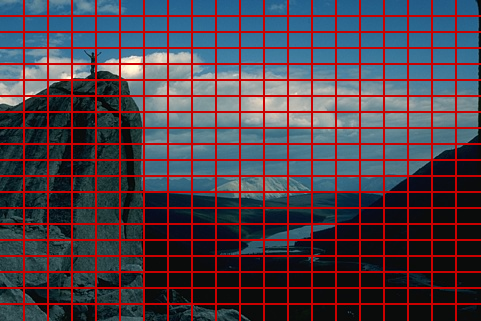
\includegraphics[scale=\scalefivebsd]{pictures/bsd-1-seeds-level-4}
	}
	\subfigure{
		\label{subfig:superpixel-segmentation-seeds-blocks-level-3}
		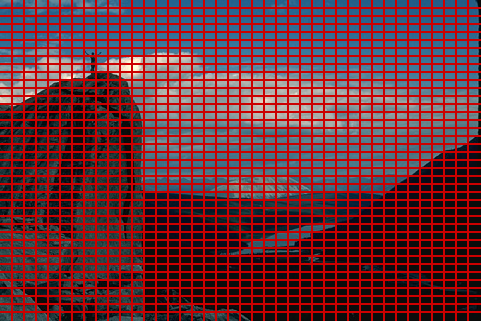
\includegraphics[scale=\scalefivebsd]{pictures/bsd-1-seeds-level-3}
	}
%	\subfigure[Blocks at level $l = 2$.]{
%		\label{subfig:superpixel-segmentation-seeds-blocks-level-2}
%		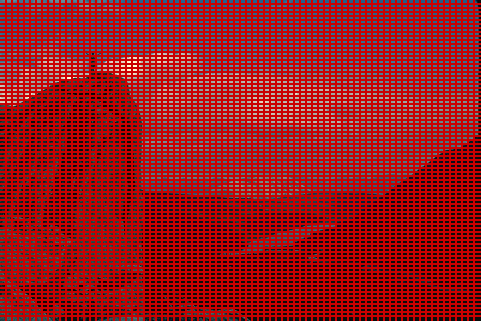
\includegraphics[scale=\scalethreebsd]{pictures/bsd-1-seeds-level-2}
%	}
	\subfigure{
		\label{subfig:superpixel-segmentation-seeds-blocks-after-3}
		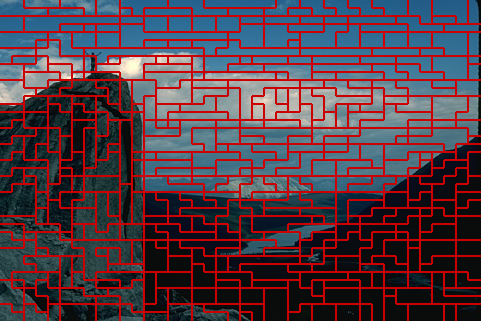
\includegraphics[scale=\scalefivebsd]{pictures/bsd-1-seeds-after-3}
	}
	\subfigure{
		\label{subfig:superpixel-segmentation-seeds-blocks-after-2}
		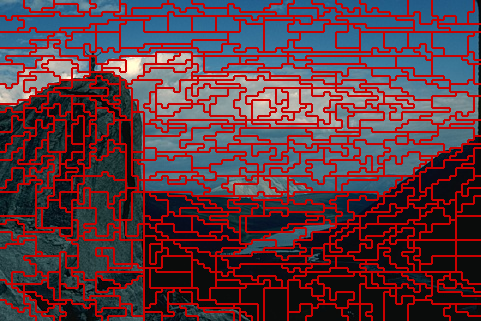
\includegraphics[scale=\scalefivebsd]{pictures/bsd-1-seeds-after-2}
	}
	\subfigure{
		\label{subfig:superpixel-segmentation-seeds-blocks-after-1}
		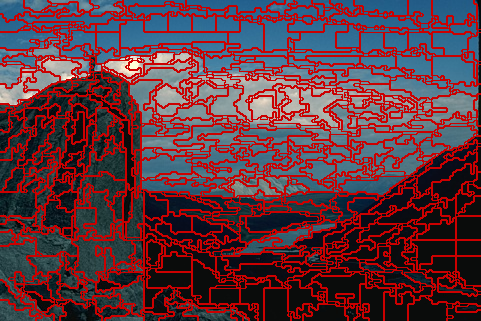
\includegraphics[scale=\scalefivebsd]{pictures/bsd-1-seeds-after-1}
	}
	\caption[An illustration of the block hierarchy used by \textbf{SEEDS} \cite{VanDenBerghBoixRoigCapitaniVanGool:2012} to exchange blocks between superpixels of an initial superpixel segmentation.]{Using $w^{(1)} = 3$, $h^{(1)} = 2$ and $L = 4$ which results in $400$ superpixels, from left to right: the block segmentation at level $l = 4$; the block segmentation at level $l = 3$; the superpixel segmentation after performing block updates at level $l = 3$; the superpixel segmentation after performing block updates at level $l = 2$ and the superpixel segmentation before performing pixel updates, that it after performing block updates at level $l = 1$.}
	\label{fig:superpixel-segmentation-seeds-blocks}
\end{figure}

As alternative to pixel updates based on color histograms, Van den Bergh \etal \cite{VanDenBerghBoixRoigCapitaniVanGool:2012} propose so called mean pixel updates. The similarity of pixel $x_n$ and superpixel $S_j$ is then expressed as euclidean distance in color space:
\begin{align}
	\label{eq:superpixel-segmentation-seeds-distance}
	d(x_n,S_j) = \| I(x_n) - I(S_j)\|_2.
\end{align}
Each pixel $x_n$ gets assigned to the superpixel minimizing the above distance, see algorithm \ref{algo:superpixel-segmentation-seeds-mean-pixel-updates}. We use \textbf{SEEDSmp} to refer to \textbf{SEEDS} using mean pixel updates.
\begin{algorithm}[t]
	\begin{algo}{SEEDS}{\label{algo:superpixel-segmentation-seeds-mean-pixel-updates}\qinput{color image $I$, initial superpixel segmentation $S$}\qoutput{superpixel segmentation $S$}}
		\qfor $k = 1$ \qto $K$\\
			initialize mean $I(S_k)$\qrof\\
		\qcom{Mean pixel updates:}\\
		\qfor $n = 1$ \qto $N$\\
			let $S_j$ be the superpixel $x_n$ belongs to\\
			\qif a neighboring pixel belongs to a different superpixel $S_k$\\
				\qthen\qif $d(x_n, S_k) < d(x_n, S_j)$\label{line:superpixel-segmentation-seeds-mean-pixel-criterion}\\
					\qthen $S_k$ \qlet $S_k \cup \{x_n\}$ and $S_j$ \qlet $S_j - \{x_n\}$\qfi\qfi\qrof\\
		\qreturn $S$
	\end{algo}
	\caption[As alternative to pixel updates as described in algorithm \ref{algo:superpixel-segmentation-seeds}, Van den Bergh \etal \cite{VanDenBerghBoixRoigVanGool:2013} propose mean pixel updates.]{As alternative to pixel updates as described in algorithm \ref{algo:superpixel-segmentation-seeds}, Van den Bergh \etal \cite{VanDenBerghBoixRoigVanGool:2013} propose mean pixel updates. This variant of \textbf{SEEDS} is referred to as \textbf{SEEDSmp}.}
	\label{fig:superpixel-segmentation-seeds-mean-pixel-updates}
\end{algorithm}

As compact and smooth superpixels may be preferable \cite{SchickFischerStiefelhagen:2012}, a smoothing term can be integrated into pixel updates. Therefore, we consider a local neighborhood around each pixel pair $(x_n,x_m)$ belonging to different superpixels $S_j$ and $S_k$, respectively. Let $N_1(x_n,x_m)$ denote the $3 \times 4$ or $4 \times 3$ neighborhood around the pixel pair $(x_n, x_m)$. %, see \ref{fig:superpixel-segmentation-seeds-smoothing}.
%\begin{figure}
%	\begin{tikzpicture}
%		\draw[dotted](-0.5,0) -- (0,0);\draw (0,0) -- (2,0);\draw[dotted](2,0) -- (2.5,0);
%		\draw[dotted](-0.5,0.5) -- (0,0.5);\draw (0,0.5) -- (2,0.5);\draw[dotted](2,0.5) -- (2.5,0.5);
%		\draw[dotted](0.5,-1) -- (0.5,-0.5);\draw (0.5,-0.5) -- (0.5,1);\draw[dotted](0.5,1) -- (0.5,1.5);
%		\draw[dotted](1,-1) -- (1,-0.5);\draw (1,-0.5) -- (1,1);\draw[dotted](1,1) -- (1,1.5);
%		\draw[dotted](1.5,-1) -- (1.5,-0.5);\draw (1.5,-0.5) -- (1.5,1);\draw[dotted](1.5,1) -- (1.5,1.5);
%	\end{tikzpicture}
%	\label{fig:superpixel-segmentation-seeds-smoothing}
%\end{figure}
If the number of pixels $N_{n,m,k}$ within $N_1(x_n,x_m)$ belonging to superpixel $S_k$ is greater than the number of pixels $N_{n,m,j}$ belonging to superpixel $S_j$, pixel $x_n$ is more likely to belong to superpixel $S_k$ as well\footnote{In practice, the pixel to be exchanged is not considered within the counts $N_{n,m,k}$ and $N_{n,m,j}$.} \cite{VanDenBerghBoixRoigCapitaniVanGool:2012}. The criterion for pixel updates given in line \ref{line:superpixel-segmentation-seeds-pixel-criterion} of algorithm \ref{algo:superpixel-segmentation-seeds} changes to
\begin{align}
	\label{eq:superpixle-segmentation-seeds-original-smoothing}
	N_{n,m,k} \cdot h_{S_k}(h(x_n)) > N_{n,m,j} \cdot h_{S_j}(h(x_n)).
\end{align}
For mean pixel updates as given in algorithm \ref{algo:superpixel-segmentation-seeds-mean-pixel-updates}, line \ref{line:superpixel-segmentation-seeds-mean-pixel-criterion} changes to
\begin{align}
	\label{eq:superpixle-segmentation-seeds-original-smoothing-mean}
	\frac{d(x_n,S_k)}{N_{n,m,k}} < \frac{d(x_n, S_j)}{N_{n,m,j}}.
\end{align}

An alternative smoothing term \cite{VanDenBerghBoixRoigVanGool:2013} uses the pixel coordinates to redefine the distance given in equation \eqref{eq:superpixel-segmentation-seeds-distance} as
\begin{align}
	\label{eq:superpixel-segmentation-seeds-spatial-smoothing}
	d(x_n,S_j) = \| I(x_n) - I(S_j)\|_2 + \beta\|x_n - \mu(S_j)\|_2.
\end{align}
where $\beta$ controls the compactness of the generated superpixels. Note that both smoothing terms can also be combined. With \textbf{SEEDSmp*} we refer to \textbf{SEEDS} using mean pixel updates and the alternative smoothing term of equation \eqref{eq:superpixel-segmentation-seeds-spatial-smoothing}.

\subsection{Complexity}
\label{subsection:superpixel-segmentation-seeds-complexity}

In the following we give a detailed analysis of the complexity of \textbf{SEEDS}. For initialization, we first run over all pixels to compute the corresponding histogram bins and then compute the histograms for level $l = 1$. Computing the histogram bins for each pixel can be done in $\mathcal{O}(N)$ operations using uniform binning or in $\mathcal{O}(3N + 255Q)$ operations using non-uniform binning based on integral channels\footnote{For each $8$-bit channel of the color image $I$, the corresponding integral channel represents an array where the $i^{\text{th}}$ entry, $0 \leq i \leq 255$, counts the number of pixels whose color in this channel is equal or smaller than $i$. Then, non-uniform binning chooses the bins such that approximately the same number of pixels fall in each bin.}. Together, this requires
\begin{align}
	\label{eq:superpixel-segmentation-seeds-complexity-initialization-1}
	3N + 255Q + \floor*{\frac{W}{w^{(1)}}} \cdot \floor*{\frac{H}{h^{(1)}}} \cdot w^{(1)} \cdot h^{(1)} = \mathcal{O}(4N + 255Q)
\end{align}
operations. The histograms at level $1 < l \leq L$ can be computed as the sum of the corresponding histograms at level $(l - 1)$: four blocks at level $(l - 1)$ form a block at level $l$. Then the initialization of the histograms for all levels $1 < l \leq L$ requires
\begin{align}
	\label{eq:superpixel-segmentation-seeds-complexity-initialization-l}
	\sum_{l = 2}^L 4\cdot \floor*{\frac{W}{w^{(l)}}} \cdot \floor*{\frac{H}{h^{(l)}}} \cdot Q \approx \sum_{l = 2}^L 4 \cdot \frac{N}{w^{(l)} h^{(l)}} \cdot Q
\end{align}
operations. Considering $w^{(1)} \geq 2$ and $h^{(1)} \geq 2$, equations \eqref{eq:superpixel-segmentation-seeds-complexity-initialization-1} and \eqref{eq:superpixel-segmentation-seeds-complexity-initialization-l} are at most linear in the number of pixels: $\mathcal{O}(4QN)$.

For block updates at level $1 \leq l < L$ we consider the worst case: each block has four neighbors belonging to different superpixels. Then, we need to compute the histogram intersection five times: four times for the neighboring superpixels, once for the current superpixel. Overall, for block updates at all levels $1 \leq l < L$, this results in
\begin{align}
	\label{eq:superpixel-segmentation-seeds-complexity-block-updates}
	\sum_{l = 1}^{L - 1} 5 \cdot \floor*{\frac{W}{w^{(l)}}} \cdot \floor*{\frac{H}{h^{(l)}}} \cdot Q \approx \sum_{l = 1}^{L - 1} 5 \cdot \frac{N}{w^{(l)}h^{(l)}} \cdot Q
\end{align}
operations. Hence, block updates at all levels $1 \leq l < L$ are linear in $N$ when considering the histogram size $Q$ to be a constant: $\mathcal{O}(5QN)$.

Considering pixel updates as in algorithm \ref{algo:superpixel-segmentation-seeds}, for each pixel we need to calculate the similarity to five different superpixels: $\mathcal{O}(5N)$ operations. Considering mean pixel updates as in algorithm \ref{algo:superpixel-segmentation-seeds-mean-pixel-updates}, computing the superpixel centers can be done in $\mathcal{O}(N + K)$ operations\footnote{In practice, for each superpixel $S_k$ the sums and the normalization needed to compute the means $I(S_k)$ and $\mu(S_k)$ are stored separately, resulting in $\mathcal{O}(N)$ operations for initialization.}. Further, in the worst case, $\mathcal{O}(5N)$ operations are necessary to perform mean pixel updates.

Overall, the algorithm has linear runtime in the number of pixels. However, for block updates, the number of histogram bins plays an important role. In addition, both block and pixel updates are in practice iterated more than once, such that the number of iterations $T$ influences the runtime as well: $\mathcal{O}(QTN)$. While this describes the worst case, we note that in practice, the runtime is also influenced by the number of levels $L$ and the block size $w^{(1)} \times h^{(1)}$.

\subsection{Theoretical Background}

We follow \cite{VanDenBerghBoixRoigCapitaniVanGool:2012} to derive the energy which Van den Bergh \etal aim to maximize using algorithm~\ref{algo:superpixel-segmentation-seeds}. The energy comprises a color term $H(S)$ and a smoothing term $B(S)$:
\begin{align}
	\label{eq:superpixel-segmentation-seeds-objective-function}
	E(S) = H(S) + \lambda B(S).
\end{align}
where $\lambda$ is a balancing parameter. In practice, $\lambda$ is not adaptable as the smoothing term introduced in equation \eqref{eq:superpixle-segmentation-seeds-original-smoothing} does not allow to adapt its importance.

The color term favors superpixels with color histograms concentrated in a single bin. Therefore, a color term of the form
\begin{align}
	\label{eq:superpixel-segmentation-seeds-color-term}
	H(S) = \sum_{S_j \in S} \sum_{q = 1} ^Q h_{S_j}(q)^2
\end{align}
is used. As of equation \eqref{eq:superpixel-segmentation-seeds-color-term}, $H(S)$ reaches its maximum if and only if each superpixel histogram is concentrated in a single bin \cite{VanDenBerghBoixRoigCapitaniVanGool:2012}. As alternative, Van den Bergh \etal refer to an entropy based color term\footnote{That is, $H(S) = - \sum_{S_j \in S} \sum_{q = 1} ^Q h_{S_j}(q) \log(h_{S_j}(q))$ where the histogram $h_{S_j}$ is interpreted as discrete probability distribution.}. Another possible color term is given by
\begin{align}
	H(S) = \sum_{S_j \in S} \max_q \{h_{S_j}(q)\},
\end{align}
favoring histograms concentrated in a single bin as well.

The boundary term is based on superpixel histograms. For each pixel $x_n$, the corresponding superpixel histogram $g_{x_n}$ counts the number of pixels $x_m \in N_R(x_n)$ belonging to each superpixel $1 \leq k \leq K$. Then, the boundary term is given by
\begin{align}
	B(S) = \sum_{n = 1}^N \sum_{k = 1} ^K g_{x_n}(k)^2.
\end{align}
This boundary term favors regular superpixels with smooth borders: When considering the superpixel histograms of all pixels within a specific superpixel, the superpixel histograms of pixels lying at the border will never be concentrated in one bin. However, with a more compact form of the superpixel, more pixels will have a uniformly labeled neighborhood, maximizing $B(S)$ \cite{VanDenBerghBoixRoigCapitaniVanGool:2012}.

To implement a hill climbing algorithm maximizing the energy $E(S)$, Van den Bergh \etal proof the following propositions:
\begin{prop}
	\label{prop:superpixel-segmentation-seeds-prop-1}
	Let $S_j$, $S_k$ be superpixels similar in size, and the size of block $B_i^{(l)} \subseteq S_j$ be much smaller: $|B_i^{(l)}| \ll |S_j| \approx |S_k|$. Let $S$ denote the current superpixel segmentation and $S_p$ denote the proposed superpixel segmentation where block $B_i^{(l)}$ is moved to superpixel $S_k$. If the color histogram $h_{B_i^{(l)}}$ is concentrated in one bin, it holds:
	\begin{align}
		\cap (h_{B_i^{(l)}}, h_{S_k}) \geq \cap (h_{B_i^{(l)}}, h_{S_j - B_i^{(l)}}) \Leftrightarrow H(S_p) \geq H(S)
	\end{align}
	where $h_{S_j - B_i^{(l)}}$ is the color histogram computed over the pixels in $S_j - B_i^{(l)}$.
\end{prop}
\begin{prop}
	\label{prop:superpixel-segmentation-seeds-prop-2}
	Let $x_n$ be a pixel belonging to superpixel $S_j$. Let $S$ denote the current superpixel segmentation and $S_p$ denote the proposed superpixel segmentation where $x_n$ is moved to superpixel $S_k$. Further, let $M_{x_n}$ be the set of all pixels $x_m$ for which $x_n \in N_R(x_m)$, then it holds:
	\begin{align}
		\sum_{x_m \in M_{x_n}} (g_{x_m}(k) + 1) \geq \sum_{x_m \in M_{x_n}} g_{x_m}(j) \Leftrightarrow G(S_p) \geq G(S).
	\end{align}
\end{prop}
\noindent Algorithm \ref{algo:superpixel-segmentation-seeds} is intended to maximize $E(S)$ via hill climbing: In each step, a new superpixel segmentation is proposed by exchanging blocks or pixels and the proposed superpixels segmentation is accepted if the energy increases.

\subsection{Discussion}

Although the implementation provided by Van den Bergh \etal performs well, the implementation lacks relation to the theoretical background discussed in the previous section. Firstly, proposition~\ref{prop:superpixel-segmentation-seeds-prop-1} assumes the superpixel sizes to be comparable and the histogram $h_{B_i^{(l)}}$ to be concentrated in a single bin. Arguing that this holds in 93\% of the cases \cite{VanDenBerghBoixRoigCapitaniVanGool:2012}, this can merely be seen as heuristic rather than mathematical accurate. Secondly, our experiments show that the energy given in equation \eqref{eq:superpixel-segmentation-seeds-objective-function} is unsuited for superpixel segmentation in the first place. Even though, an implementation directly maximizing $E(S)$ through hill climbing may be inefficient, figure \ref{fig:superpixel-segmentation-seeds-objective-function} presents superpixel segmentations obtained from a naive implementation.
\begin{figure}[t]
	\centering
	\subfigure{
		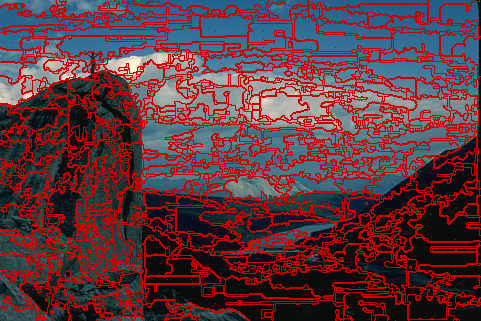
\includegraphics[scale=\scalefivebsd]{pictures/bsd-1-seeds-direct}
	}
	\subfigure{
		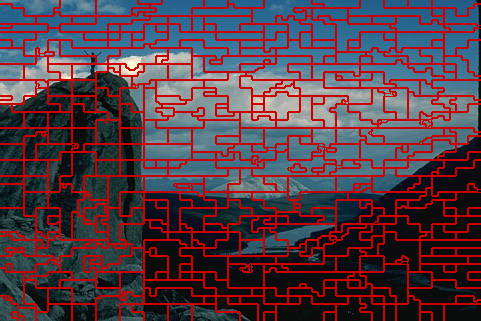
\includegraphics[scale=\scalefivebsd]{pictures/bsd-1-seeds-direct-after-1}
	}
	\subfigure{
		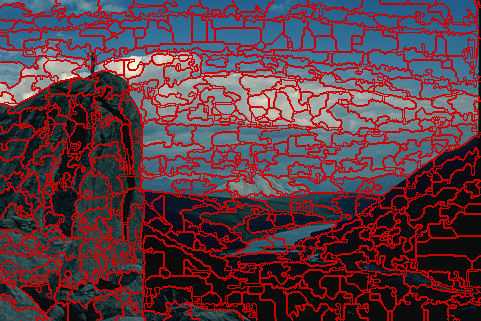
\includegraphics[scale=\scalefivebsd]{pictures/bsd-1-seeds-direct-original-pixels}
	}
	\caption[Superpixel segmentations generated by directly maximizing the energy proposed in \cite{VanDenBerghBoixRoigCapitaniVanGool:2012}.]{An illustration of the poor superpixel segmentations obtained by directly maximizing the proposed energy $E(S)$ given by equation \eqref{eq:superpixel-segmentation-seeds-color-term}. From left to right: the superpixel segmentation obtained after maximizing $E(S)$ directly using both block updates as well as pixel updates; the superpixel segmentation obtained after performing block updates at level $l = 1$ to directly maximize the energy $E(S)$; and the superpixel segmentation obtained after using block updates to optimize the energy $E(S)$ directly while using the pixel updates described in algorithm \ref{algo:superpixel-segmentation-seeds}.}
	\label{fig:superpixel-segmentation-seeds-objective-function}
\end{figure}
These experiments indicate that the idea of color histograms being concentrated in a single bin has to be relaxed in order to obtain proper superpixel segmentations. Thirdly, considering the smoothing term of the energy in equation \eqref{eq:superpixel-segmentation-seeds-objective-function}, the weight $\lambda$ cannot be adapted. Although this could be fixed by adapting equations \eqref{eq:superpixle-segmentation-seeds-original-smoothing} and \eqref{eq:superpixle-segmentation-seeds-original-smoothing-mean}, our experiments indicate that using the alternative smoothing term of equation \eqref{eq:superpixel-segmentation-seeds-spatial-smoothing} results in more compact and regular superpixels. Furthermore, mean pixel updates which are reported to give superior performance \cite{VanDenBerghBoixRoigVanGool:2013} do not conform to the theoretical background introduced in the previous section.
\begin{figure}[b]
	\centering
	\subfigure{
		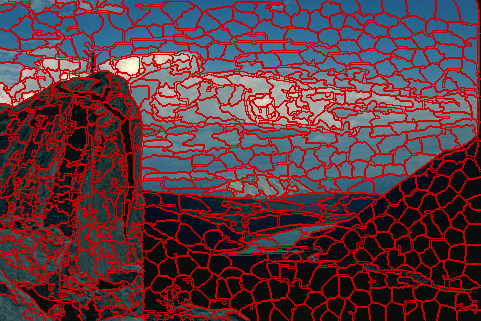
\includegraphics[scale=\scalefivebsd]{pictures/bsd-1-reseedssm}
	}
	\subfigure{
		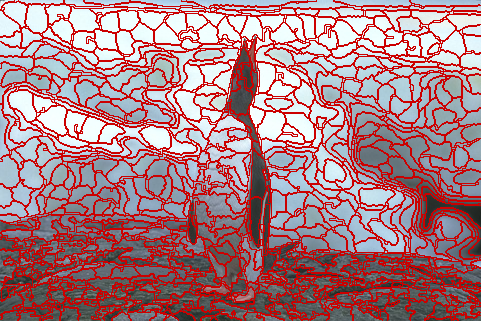
\includegraphics[scale=\scalefivebsd]{pictures/bsd-2-reseedssm}
	}
	\subfigure{
		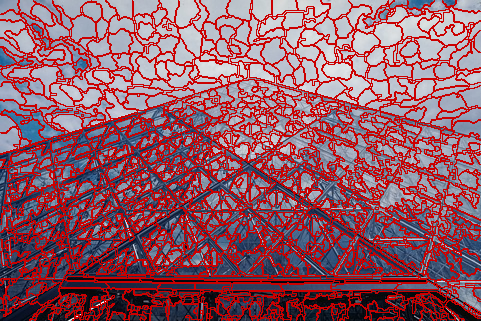
\includegraphics[scale=\scalefivebsd]{pictures/bsd-3-reseedssm}
	}
	\subfigure{
		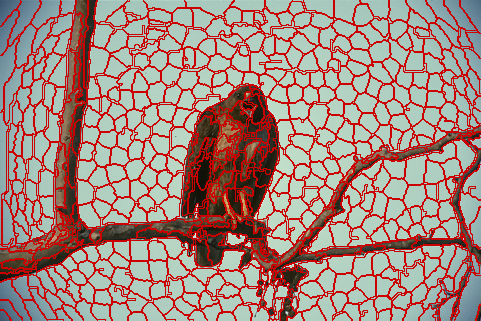
\includegraphics[scale=\scalefivebsd]{pictures/bsd-4-reseedssm}
	}
	\subfigure{
		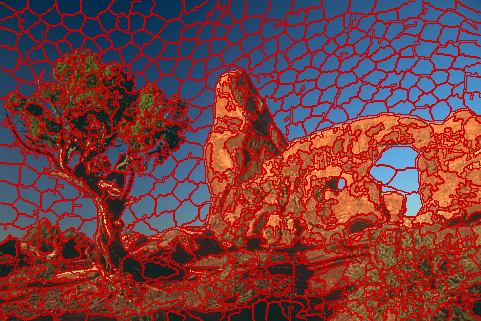
\includegraphics[scale=\scalefivebsd]{pictures/bsd-5-reseedssm}
	}
	\caption[Superpixel segmentations obtained from our implementation of \textbf{SEEDS} \cite{VanDenBerghBoixRoigCapitaniVanGool:2012} using mean pixel updates and the alternative smoothing term of equation \eqref{eq:superpixel-segmentation-seeds-spatial-smoothing}.]{The running examples oversegmented into exactly $600$ superpixels using our implementation of \textbf{SEEDS} using mean pixel updates and the alternative smoothing term of equation \eqref{eq:superpixel-segmentation-seeds-spatial-smoothing} which we refer to as \textbf{SEEDSmp*}. Further examples can be found in section \ref{subsection:evaluation-comparison-qualitative} and appendix \ref{chapter:appendix-evaluation}.}
	\label{fig:superpixel-segmentation-seeds-results}
\end{figure}
Overall, figure \ref{fig:superpixel-segmentation-seeds-results} shows the running examples oversegmented using our implementation with mean pixel updates as well as the alternative smoothing term of equation \eqref{eq:superpixel-segmentation-seeds-spatial-smoothing}. In conclusion, we find the theoretical background of \textbf{SEEDS} as provided by Van den Bergh \etal \cite{VanDenBerghBoixRoigCapitaniVanGool:2012} unsuited in the light of the provided implementation and our experiments. However, a novel formulation of \textbf{SEEDS} lies not within the scope of this thesis.

\subsection{Implementation Details}

Our implementation of \textbf{SEEDS} closely follows algorithm \ref{algo:superpixel-segmentation-seeds}. The histograms are pre-computed for all blocks across all levels. This can be done efficiently by accumulating histograms of level $(l - 1)$ to form the histograms in level $1 < l \leq L$. The original implementation, as well as our implementation, both use non-uniform binning, that is the bin size is adapted to the colors present within the image. Then, the histograms only need to be updated after exchanging blocks or pixels. When using mean pixel updates as in algorithm \ref{algo:superpixel-segmentation-seeds-mean-pixel-updates}, the superpixel centers need to be computed just before starting pixel updates. In practice the individual terms of equation \eqref{eq:superpixel-segmentation-seeds-spatial-smoothing} can also be normalized in order to choose the weighting parameter $\beta$ more easily.

\section{SLIC}
\label{section:superpixel-segmentation-slic}

\textbf{SLIC} is a gradient ascent method growing superpixels from initial superpixel centers using color similarity and spatial proximity. In particular, \textbf{SLIC} performs local $K$-means clustering where the search space for each superpixel is restricted to a local neighborhood around its center. The approach is easily implemented and adapted to custom needs. In addition, it can naturally be extended to depth or video data and is commonly used for comparison. We revisit the algorithm in detail and give a brief discussion.

% \textbf{SLIC} is a gradient ascent approach, as well, and comparable to a local $K$-means clustering (\eg see \cite{Bishop:2006} for details on $K$-means clustering). It is fast because the search space for each superpixel is limited to a local neighborhood. We revisit the algorithm before giving a short discussion. For this thesis, \textbf{SLIC} is of interest as it implements a superpixel algorithm easily extendable to using depth information (see chapter \ref{chapter:superpixel-segmentation-depth}) and as it is commonly used as baseline.

\subsection{Algorithm}

The algorithm can be described as local $K$-means clustering in a five dimensional space comprising pixel coordinates and color \cite{AchantaShajiSmithLucchiFuaSuesstrunk:2010}, see algorithm \ref{algo:superpixel-segmentation-slic}.
\begin{algorithm}[t!]
	\begin{algo}{SLIC}{\label{algo:superpixel-segmentation-slic}\qinput{color image $I$, number of superpixels $K$}\qoutput{superpixel segmentation $S$}}
		initialize superpixel centers on a regular grid with step size $R$\\
		move centers to low-gradient magnitude positions\\
		\qrepeat\\
			\qfor $k = 1$ \qto $K$\\
				\qforeach pixel $x_n$ in a $2R \times 2R$ neighborhood around $\mu(S_k)$\\
					\qif $x_n$ is unassigned\\
						\qthen $S_k$ \qlet $S_k \cup \{x_n\}$\qfi\\
					\qelseif $d(x_n, S_k) < d(x_n, S_{s(x_n)})$\\
						\qthen $S_k$ \qlet $S_k \cup \{x_n\}$ and $S_{s(x_n)}$ \qlet $S_{s(x_n)} - \{x_n\}$\qfi\qrof\qrof
		\quntil nothing changes \qcom{or maximum number of iterations reached.}\\
		enforce connectivity\\
		\qreturn $S$
	\end{algo}
	\caption[The basic algorithm of \textbf{SLIC} \cite{AchantaShajiSmithLucchiFuaSuesstrunk:2010}.]{\textbf{SLIC} is implemented as local $K$-means clustering. Here, local means that for each superpixel only pixels in a $2R \times 2R$ window around the superpixel's center are of interest. After clustering, \textbf{SLIC} needs to enforce connectivity.}
	\label{fig:superpixel-segmentation-slic-algorithm}
\end{algorithm}
The superpixel centers are initialized on a regular grid with step size $R$. In practice, the centers are then moved to locations with low gradient magnitude to avoid placing superpixel centers at strong edges. The step size of the regular grid can be computed as
\begin{align}
	R = \floor*{\frac{WH}{K}}.
\end{align}
Then, each pixel $x_n$ gets assigned to the nearest superpixel with respect to the following distance:
\begin{align}
	\label{eq:superpixel-segmentation-slic-distance}
	d(x_n, S_j) = \|I(x_n) - I(S_j)\|_2 + \frac{\beta}{R} \|x_n - \mu(S_j)\|_2
\end{align}
where $\beta$ is a parameter controlling the compactness. However, in contrast to classical $K$-means clustering, for each superpixel only pixels in a $2R \times 2R$ neighborhood around the superpixel's center are of interest. Afterwards, the superpixel centers are updated according to the new assignment. This procedure is iterated until convergence or for a maximum number of $T$ iterations. Finally, superpixels do not necessarily represent connected components such that \textbf{SLIC} needs to enforce connectivity after clustering.

\subsection{Theoretical Background}

In general, $K$-means clustering minimizes an energy given by
\begin{align}
	\label{eq:superpixel-segmentation-slic-objective}
	E(S) = \sum_{S_j \in S} \sum_{n = 1}^N a_{n,j} d(x_n, S_j)^2
\end{align}
where $a_{n,j} = 1$ if and only if pixel $x_n$ is assigned to superpixel $S_j$, else $a_{n,j} = 0$. However, \textbf{SLIC} relaxes this energy in that the search space for each superpixel is restricted to a $2R \times 2R$ neighborhood around $\mu(S_j)$. Therefore, for fixed $\mu(S_j)$, the energy can be rewritten as
\begin{align}
	E(S) = \sum_{S_j \in S} \sum_{x_n \in N_{2R}(\mu(S_j))} a_{n,j} d(x_n, S_j)^2.
\end{align}
Additionally, the above energy is not minimized subject to the constraint that the superpixels $S_j$ are connected components. Therefore, the last step of enforcing connectivity may actually increase the energy.

\subsection{Complexity}

While classical $K$-means clustering has complexity $\mathcal{O}(NKT)$, \textbf{SLIC} runs linear in the number of pixels because of the restricted search space: For each superpixel, only pixels in a $2R \times 2R$ neighborhood around the superpixel's center are considered. Therefore, \textbf{SLIC} has complexity $\mathcal{O}(TN)$.

\subsection{Discussion}

One advantage of \textbf{SLIC} is its simplicity and efficiency \cite{AchantaShajiSmithLucchiFuaSuesstrunk:2012}. There are several implementations available: the original implementation by Achanta \etal \cite{AchantaShajiSmithLucchiFuaSuesstrunk:2010}, an implementation as part of the VLFeat Library \cite{VedaldiFulkerson:2008} and a parallel GPU implementation by Ren and Reid \cite{RenReid:2011}. Further, \textbf{SLIC} can easily be adapted by changing the distance in equation \eqref{eq:superpixel-segmentation-slic-distance}. For example, Schick \etal improve the balancing between color and spatial term by changing equation \eqref{eq:superpixel-segmentation-slic-distance} to
\begin{align}
	d(x_n, S_j) = (1 - \beta)\|I(x_n) - I(S_j)\|_2 + \frac{\beta}{R} \|x_n - \mu(S_j)\|_2.
\end{align}

On the other hand, \textbf{SLIC} only generates a valid superpixel segmentation after enforcing connectivity. This means, that the algorithm cannot be aborted after an arbitrary number of iterations. In addition, Van den Bergh \etal \cite{VanDenBerghBoixRoigVanGool:2013} report lower performance with more iterations which may be due to the generated ``stray labels'' \cite{VanDenBerghBoixRoigVanGool:2013} -- small groups of pixels not connected to their corresponding superpixel. This is also confirmed by Tang \etal \cite{DaiTangHuazhaFuXiaochunCao:2012} reporting only a small decrease in performance when using only $T = 1$ iteration. However, considering an approach similar to \textbf{VCCS} \cite{PaponAbramovSchoelerWoergoetter:2013} (see section \ref{section:superpixel-segmentation-depth-vccs}), breadth-first search could be used as basis for $K$-means clustering in order to avoid stray labels. To sum up, figure \ref{fig:superpixel-segmentation-slic-results} shows the running examples oversegmented using the original implementation of \textbf{SLIC}.
\begin{figure}[t]
	\centering
	\subfigure{
		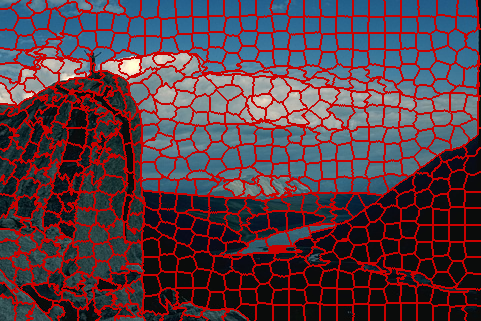
\includegraphics[scale=\scalefivebsd]{pictures/bsd-1-orislic}
	}
	\subfigure{
		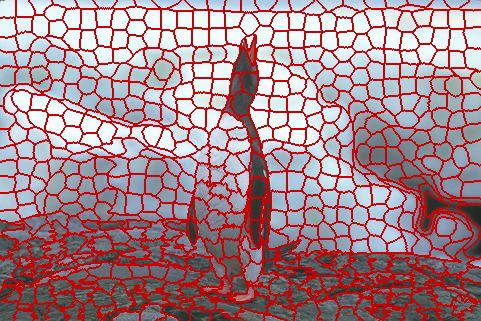
\includegraphics[scale=\scalefivebsd]{pictures/bsd-2-orislic}
	}
	\subfigure{
		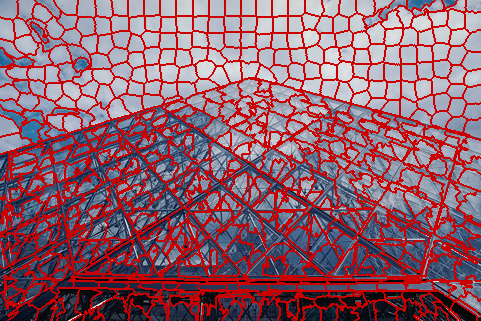
\includegraphics[scale=\scalefivebsd]{pictures/bsd-3-orislic}
	}
	\subfigure{
		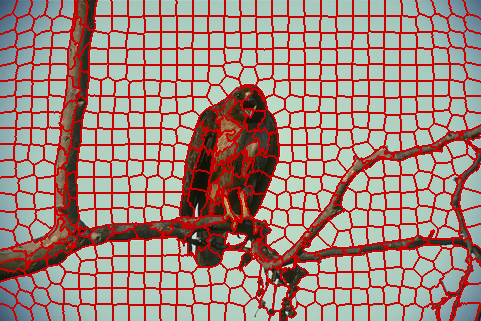
\includegraphics[scale=\scalefivebsd]{pictures/bsd-4-orislic}
	}
	\subfigure{
		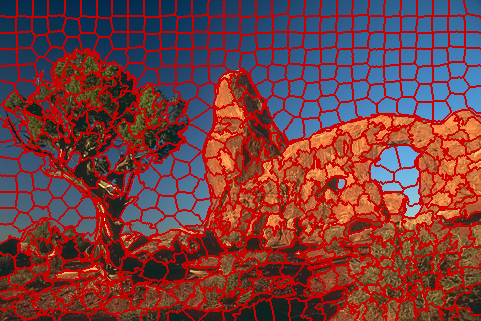
\includegraphics[scale=\scalefivebsd]{pictures/bsd-5-orislic}
	}
	\caption[Superpixel segmentations generated by the original implementation of \textbf{SLIC} \cite{AchantaShajiSmithLucchiFuaSuesstrunk:2012}.]{Superpixel segmentations with roughly $600$ superpixels of the running examples generated by the original implementation of \textbf{SLIC}. Further examples can be found in section \ref{subsection:evaluation-comparison-qualitative} and appendix~\ref{chapter:appendix-evaluation}.}
	\label{fig:superpixel-segmentation-slic-results}
\end{figure}